\documentclass{article}
\usepackage[margin=1in]{geometry} %1 in margins
\usepackage{graphicx} %For including graphics
\usepackage[labelfont=bf]{caption} %Make float labels bold
\usepackage{subcaption}
\usepackage{amsmath}    
\usepackage{listings}% http://ctan.org/pkg/listings
\usepackage{cancel}
\lstset{
  basicstyle=\ttfamily,
  mathescape
}
\usepackage{hyperref}
\renewcommand{\floatpagefraction}{0.95}
\renewcommand{\topfraction}{0.95}
\renewcommand{\textfraction}{0.05}
\usepackage{url}

% Define a ``Program'' float for code
\usepackage{verbatim} %Allow verbatim input for code
\usepackage{float} %Defining the Program environment
\floatstyle{boxed}
\newfloat{program}{htbp}{pgm}
\floatname{program}{Program}



\begin{document}

\begin{flushright}
	Mehmet Duman
\end{flushright}

\begin{center}
{\Large {\bf Solution to Homework \#6---MTH 522} }
\end{center}

{\bf Problem 1} (Chapter 7 Exercises 6):\\
In this exercise, you will further analyze the Wage data set considered throughout this chapter.
(a) Perform polynomial regression to predict "wage" using "age". Use cross-validation to select the optimal degree d for the polynomial. What degree was chosen, and how does this compare to the results of hypothesis testing using ANOVA? Make a plot of the resulting polynomial fit to the data.

Let's see the Wage dataset
Plot the "wage" an "age"

\begin{program}
	\begin{verbatim}
	> library(ISLR)
	> library(boot)
	> set.seed(1)
	> summary(Wage)
	year           age               sex                    maritl           race     
	Min.   :2003   Min.   :18.00   1. Male  :3000   1. Never Married: 648   1. White:2480  
	1st Qu.:2004   1st Qu.:33.75   2. Female:   0   2. Married      :2074   2. Black: 293  
	Median :2006   Median :42.00                    3. Widowed      :  19   3. Asian: 190  
	Mean   :2006   Mean   :42.41                    4. Divorced     : 204   4. Other:  37  
	3rd Qu.:2008   3rd Qu.:51.00                    5. Separated    :  55                  
	Max.   :2009   Max.   :80.00                                                           
	
	education                     region               jobclass   
	1. < HS Grad      :268   2. Middle Atlantic   :3000   1. Industrial :1544  
	2. HS Grad        :971   1. New England       :   0   2. Information:1456  
	3. Some College   :650   3. East North Central:   0                        
	4. College Grad   :685   4. West North Central:   0                        
	5. Advanced Degree:426   5. South Atlantic    :   0                        
	6. East South Central:   0                        
	(Other)              :   0                        
	health      health_ins      logwage           wage       
	1. <=Good     : 858   1. Yes:2083   Min.   :3.000   Min.   : 20.09  
	2. >=Very Good:2142   2. No : 917   1st Qu.:4.447   1st Qu.: 85.38  
	Median :4.653   Median :104.92  
	Mean   :4.654   Mean   :111.70  
	3rd Qu.:4.857   3rd Qu.:128.68  
	Max.   :5.763   Max.   :318.34  
	
	
	> plot(age, wage)
	> dev.copy2pdf(file = "MTH522_hw6_p1a_1.pdf", width = 8, height = 6, out.type = "pdf")  
	>  dev.off()
	\end{verbatim}
\end{program}

\newpage

\begin{figure}[htb]
	\begin{center}
		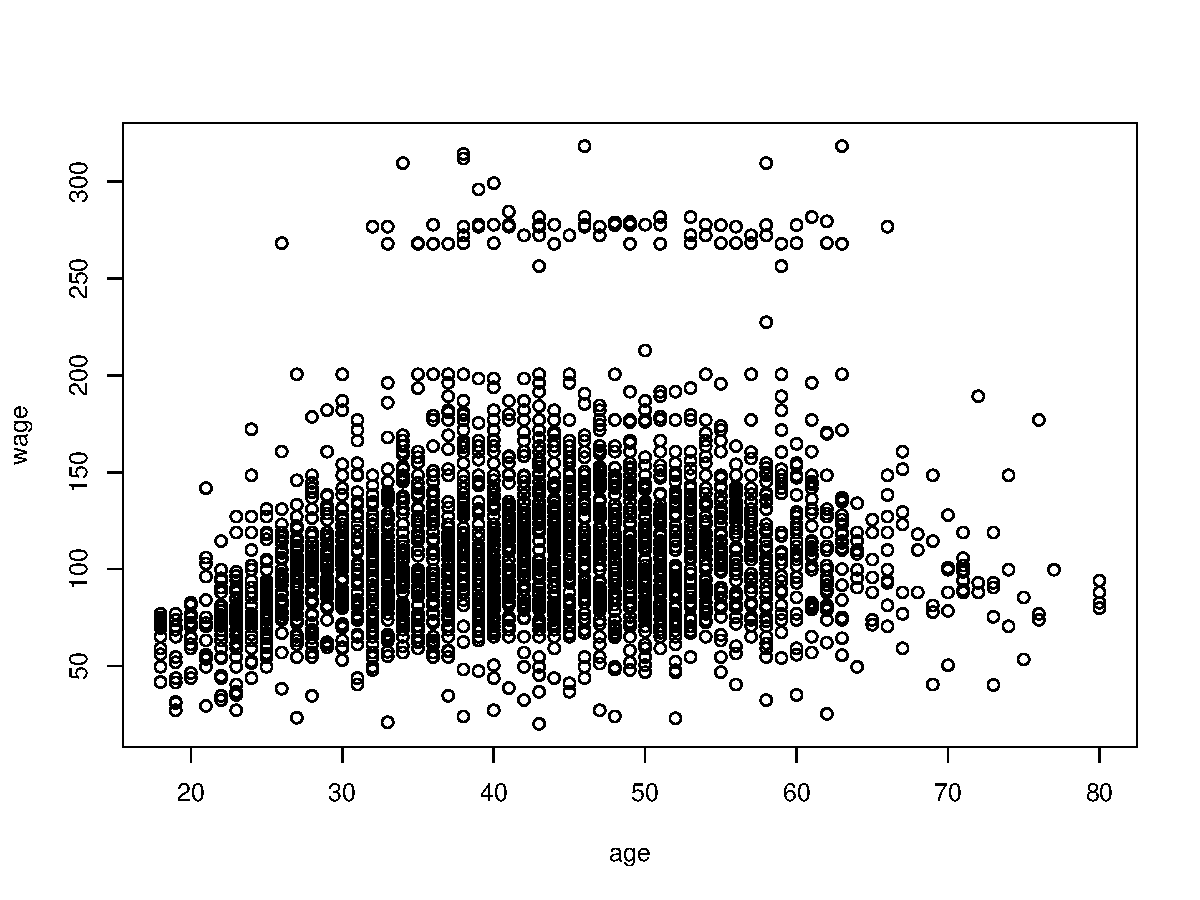
\includegraphics[width=0.8\textwidth]{MTH522_hw6_p1a_1.pdf}
	\end{center}
	\caption{.}
	\label{fig:MTH522_hw6_p1a_1}
\end{figure}

\newpage

Now, I will perform polynomial regression:

\begin{program}
	\begin{verbatim}
	> deltas = rep(0, 10)
	> for (i in 1:10) {
	+   glm.fit = glm(wage~poly(age, i), data=Wage)
	+   deltas[i] = cv.glm(Wage, glm.fit, K=10)$delta[2]
	+ }
	> plot(1:10, deltas, xlab="Degree", ylab="CV Prediction Error Estimate", type="l",
	+ pch=20 )
	>  points(which.min(deltas), deltas[which.min(deltas)], col = "red", cex = 2, pch =20)
	> dev.copy2pdf(file = "MTH522_hw6_p1a_2.pdf", width = 8, height = 6, out.type = "pdf") 
	> dev.off()

	> which.min( deltas )
	
	[1] 4
	\end{verbatim}
\end{program}
From the above plot, we can see that d=4 is the optimal degree for the polynomial, where curve stops decreasing and starts increasing.



\begin{figure}[htb]
	\begin{center}
		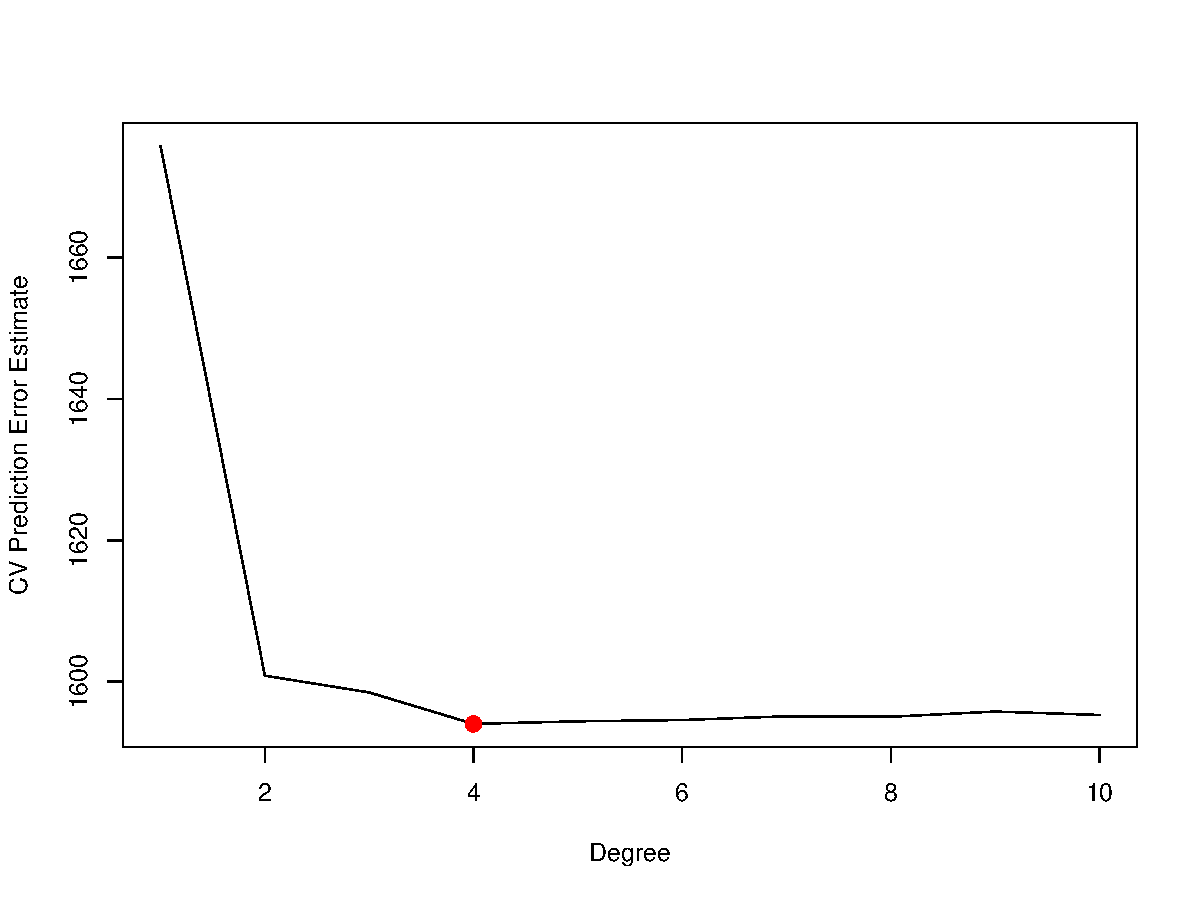
\includegraphics[width=0.8\textwidth]{MTH522_hw6_p1a_2.pdf}
	\end{center}
	\caption{.}
	\label{fig:MTH522_hw6_p1a_2}
\end{figure}

We now use ANOVA approach. The anova() function, which performs an analysis of variance (ANOVA, using an F-test) in order to test the null hypothesis that a model $M_1$ is sufficient to explain the data against the alternative hypothesis that a more complex model $M_2$ is required(Page:290)

\newpage


\begin{program}
	\begin{verbatim}
	> fit.1 = lm(wage ~ age, data=Wage)
	> fit.2 = lm(wage ~ poly(age, 2), data=Wage)
	> fit.3 = lm(wage ~ poly(age, 3), data=Wage)
	> fit.4 = lm(wage ~ poly(age, 4), data=Wage)
	> fit.5 = lm(wage ~ poly(age, 5), data=Wage)
	> anova(fit.1, fit.2, fit.3, fit.4, fit.5 )
	Analysis of Variance Table
	
	Model 1: wage ~ age
	Model 2: wage ~ poly(age, 2)
	Model 3: wage ~ poly(age, 3)
	Model 4: wage ~ poly(age, 4)
	Model 5: wage ~ poly(age, 5)
	Res.Df     RSS Df Sum of Sq        F    Pr(>F)    
	1   2998 5022216                                    
	2   2997 4793430  1    228786 143.5931 < 2.2e-16 ***
	3   2996 4777674  1     15756   9.8888  0.001679 ** 
	4   2995 4771604  1      6070   3.8098  0.051046 .  
	5   2994 4770322  1      1283   0.8050  0.369682    
	---
	Signif. codes:  0 ‘***’ 0.001 ‘**’ 0.01 ‘*’ 0.05 ‘.’ 0.1 ‘ ’ 1
	\end{verbatim}
\end{program}

As we learn from the text book (page:290), the p-value comparing the linear Model 1 to the quadratic Model 2 is essentially zero (<10−15), indicating that a linear fit is not sufficient. Similarly the p-value comparing the quadratic Model 2 to the cubic Model 3 is very low (0.0017), so the quadratic fit is also insufficient. The p-value comparing the cubic and degree-4 polynomials, Model 3 and Model 4, is ap- proximately 5 $\%$ while the degree-5 polynomial Model 5 seems unnecessary because its p-value is 0.37. Hence, either a cubic or a quartic polynomial appear to provide a reasonable fit to the data, but lower or higher order models are not justified. \\


\newpage

The polynomial prediction on the data
\begin{program}
	\begin{verbatim}
	> plot(wage~age, data=Wage, col="darkgrey")
	> agelims = range(Wage$age)
	> age.grid = seq(from=agelims[1], to=agelims[2])
	> fit = lm(wage~poly(age, 3), data=Wage)
	> pred = predict(fit, data.frame(age=age.grid))
	> lines(age.grid, pred, col="blue", lwd=2)
	> dev.copy2pdf(file = "MTH522_hw6_p1a_1.pdf", width = 8, height = 6, out.type = "pdf")  
	dev.off()
	> dev.copy2pdf(file = "MTH522_hw6_p1a_1.pdf", width = 8, height = 6, out.type = "pdf")  
	dev.off()
	> plot(wage~age, data=Wage, col="darkgrey")
	> agelims = range(Wage$age)
	> age.grid = seq(from=agelims[1], to=agelims[2])
	> fit = lm(wage~poly(age, 3), data=Wage)
	> pred = predict(fit, data.frame(age=age.grid))
	> lines(age.grid, pred, col="blue", lwd=2)
	> dev.copy2pdf(file = "MTH522_hw6_p1a_3.pdf", width = 8, height = 6, out.type = "pdf")  
	> dev.off()	
	\end{verbatim}
\end{program}



\begin{figure}[htb]
	\begin{center}
		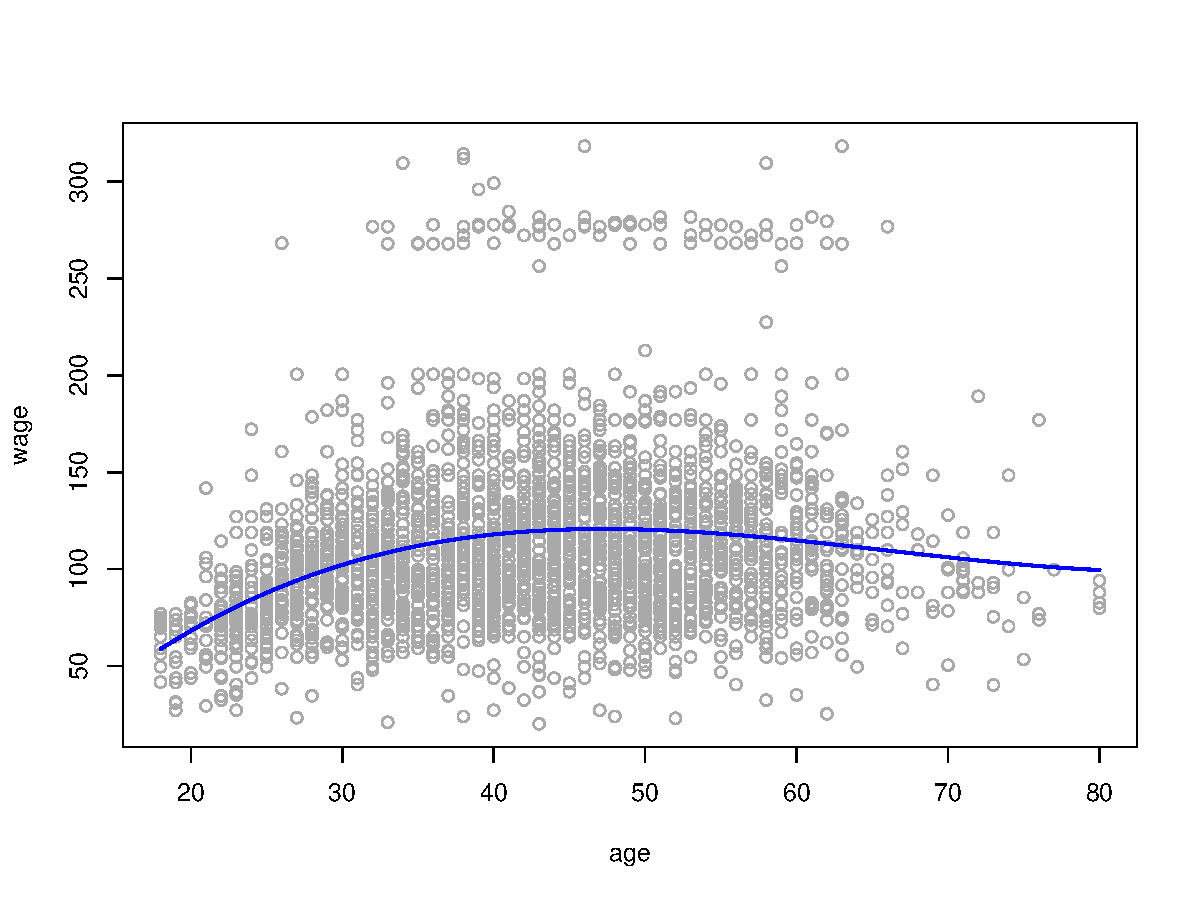
\includegraphics[width=0.8\textwidth]{MTH522_hw6_p1a_3.pdf}
	\end{center}
	\caption{.}
	\label{fig:MTH522_hw6_p1a_3}
\end{figure}

\newpage

(b) Fit a step function to predict wage using age, and perform cross-validation to choose the optimal number of cuts. Make a plot of the fit obtained.

To predict wage using age, I wil use cross-validation cut points of up to 10.

\begin{program}
	\begin{verbatim}
	> cvs = rep(NA, 10)
	> for (i in 2:10) {
	+   Wage$age.cut = cut(Wage$age, i)
	+   fit = glm(wage~age.cut, data=Wage)
	+   cvs[i] = cv.glm(Wage, fit, K=10)$delta[2]
	+ }
	> plot(2:10, cvs[-1], xlab="Cuts", ylab="CV error",
	+ type="l", pch=20, lwd=2)
	> points(which.min(cvs), cvs[which.min(cvs)], col="blue", cex=2, pch=20)
	> cvs = rep(NA, 10)
	> for (i in 2:10) {
	+   Wage$age.cut = cut(Wage$age, i)
	+   fit = glm(wage~age.cut, data=Wage)
	+   cvs[i] = cv.glm(Wage, fit, K=10)$delta[2]
	+ }
	> plot(2:10, cvs[-1], xlab="Cuts", ylab="CV error",
	+ type="l", pch=20, lwd=2)
	> points(which.min(cvs), cvs[which.min(cvs)], col="blue", cex=2, pch=20)
	> dev.copy2pdf(file = "MTH522_hw6_p1b_1.pdf", width = 8, height = 6, out.type = "pdf")  
	> dev.off()
	\end{verbatim}
\end{program}

\begin{figure}[htb]
	\begin{center}
		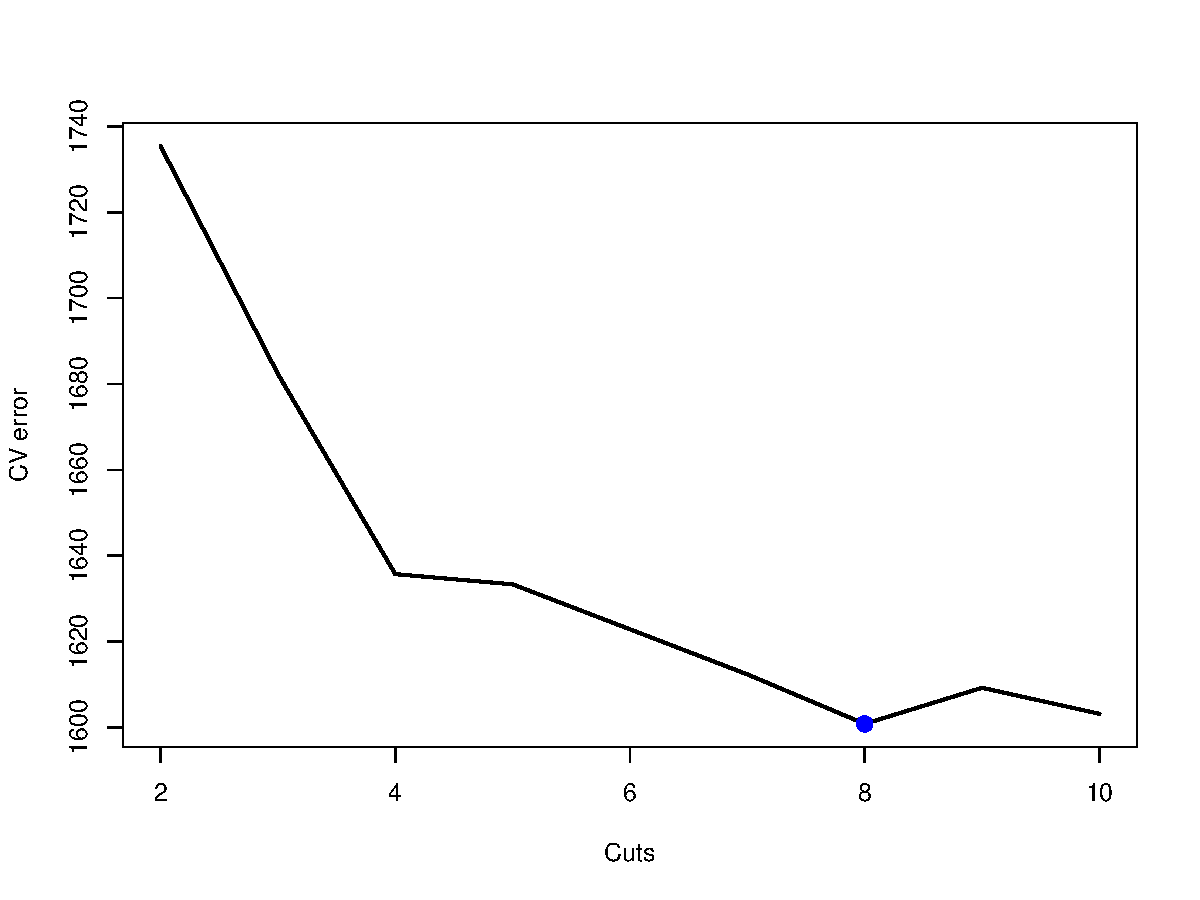
\includegraphics[width=0.8\textwidth]{MTH522_hw6_p1b_1.pdf}
	\end{center}
	\caption{.}
	\label{fig:MTH522_hw6_p1b_1}
\end{figure}

From abov plot, we can see that CV error is minimum at 8 cuts. Now we can fit dataset with step function using this 8 cuts.



\begin{program}
	\begin{verbatim}
	> fit = glm(wage~cut(age, 8), data=Wage)
	> agelims = range(Wage$age)
	> age.grid = seq(from=agelims[1], to=agelims[2])
	> pred = predict(fit, data.frame(age=age.grid))
	> plot(wage~age, data=Wage, col="darkgrey")
	> lines(age.grid, pred, col="red", lwd=2)
	> dev.copy2pdf(file = "MTH522_hw6_p1b_2.pdf", width = 8, height = 6, out.type = "pdf")
	> dev.off()
	\end{verbatim}
\end{program}

\begin{figure}[htb]
	\begin{center}
		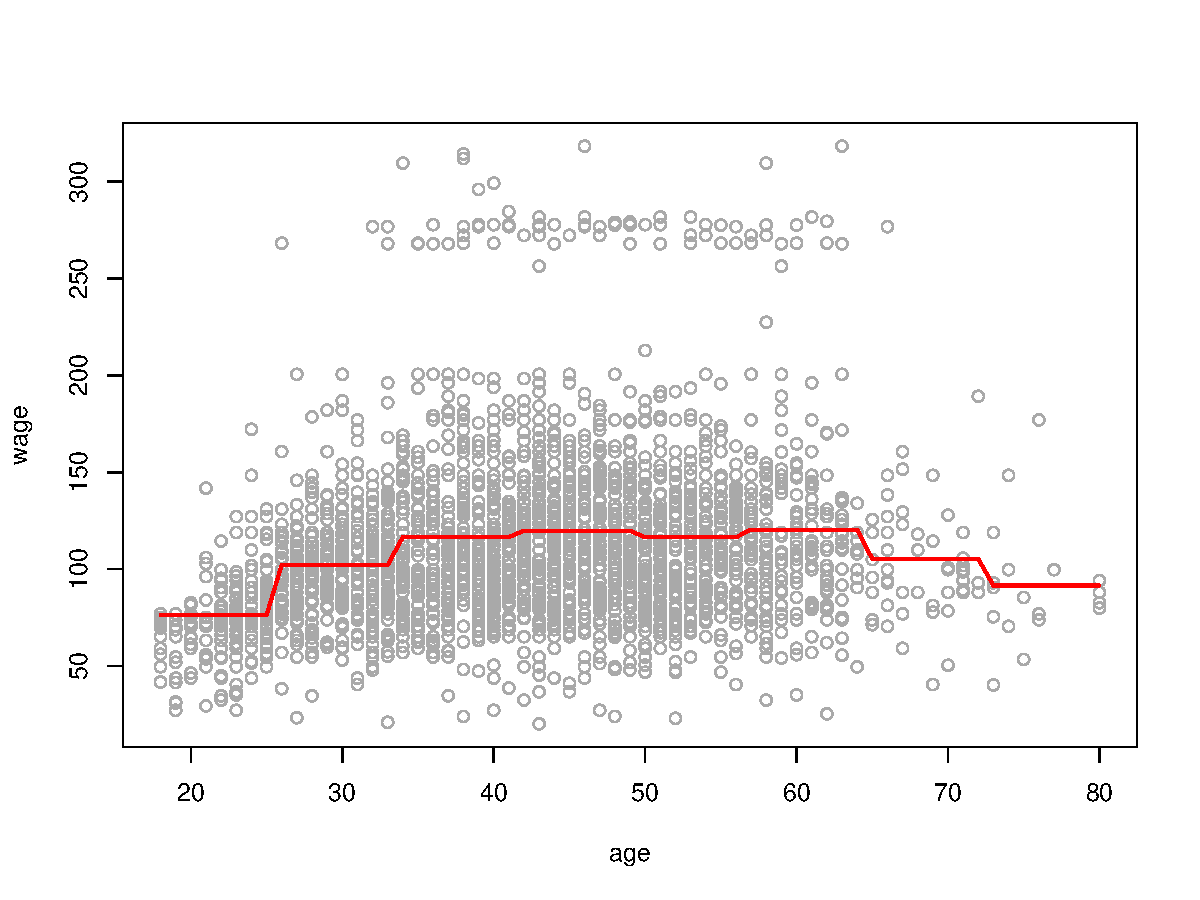
\includegraphics[width=0.8\textwidth]{MTH522_hw6_p1b_2.pdf}
	\end{center}
	\caption{.}
	\label{fig:MTH522_hw6_p1b_2}
\end{figure}


\newpage


{\bf Problem 2} (Chapter 7 Exercises 7):\\
The Wage data set contains a number of other features not explored in this chapter, such as marital status (maritl), job class (jobclass), and others. Explore the relationships between some of these other predictors and wage, and use non-linear fitting techniques in order to fit flexible models to the data. Create plots of the results obtained, and write a summary of your findings.\\



\begin{program}
	\begin{verbatim}
	> library(ISLR)
	> set.seed(1)
	> summary(Wage)
	year           age               sex                    maritl           race     
	Min.   :2003   Min.   :18.00   1. Male  :3000   1. Never Married: 648   1. White:2480  
	1st Qu.:2004   1st Qu.:33.75   2. Female:   0   2. Married      :2074   2. Black: 293  
	Median :2006   Median :42.00                    3. Widowed      :  19   3. Asian: 190  
	Mean   :2006   Mean   :42.41                    4. Divorced     : 204   4. Other:  37  
	3rd Qu.:2008   3rd Qu.:51.00                    5. Separated    :  55                  
	Max.   :2009   Max.   :80.00                                                           
	
	education                     region               jobclass   
	1. < HS Grad      :268   2. Middle Atlantic   :3000   1. Industrial :1544  
	2. HS Grad        :971   1. New England       :   0   2. Information:1456  
	3. Some College   :650   3. East North Central:   0                        
	4. College Grad   :685   4. West North Central:   0                        
	5. Advanced Degree:426   5. South Atlantic    :   0                        
	6. East South Central:   0                        
	(Other)              :   0                        
	health      health_ins      logwage           wage               age.cut   
	1. <=Good     : 858   1. Yes:2083   Min.   :3.000   Min.   : 20.09   (42.8,49]  :640  
	2. >=Very Good:2142   2. No : 917   1st Qu.:4.447   1st Qu.: 85.38   (36.6,42.8]:542  
	Median :4.653   Median :104.92   (30.4,36.6]:445  
	Mean   :4.654   Mean   :111.70   (49,55.2]  :441  
	3rd Qu.:4.857   3rd Qu.:128.68   (24.2,30.4]:347  
	Max.   :5.763   Max.   :318.34   (55.2,61.4]:270  
	(Other)    :315  
	
	\end{verbatim}
\end{program}


\newpage


\begin{program}
	\begin{verbatim}
	> par(mfrow = c(1, 2), las=2,cex.axis = 0.6)
	> plot(Wage$maritl, Wage$wage)
	> plot(Wage$jobclass, Wage$wage)
	> dev.copy2pdf(file = "MTH522_hw6_p2_1.pdf", width = 8, height = 6, out.type = "pdf")
	> dev.off()
	\end{verbatim}
\end{program}

\begin{figure}[htb]
	\begin{center}
		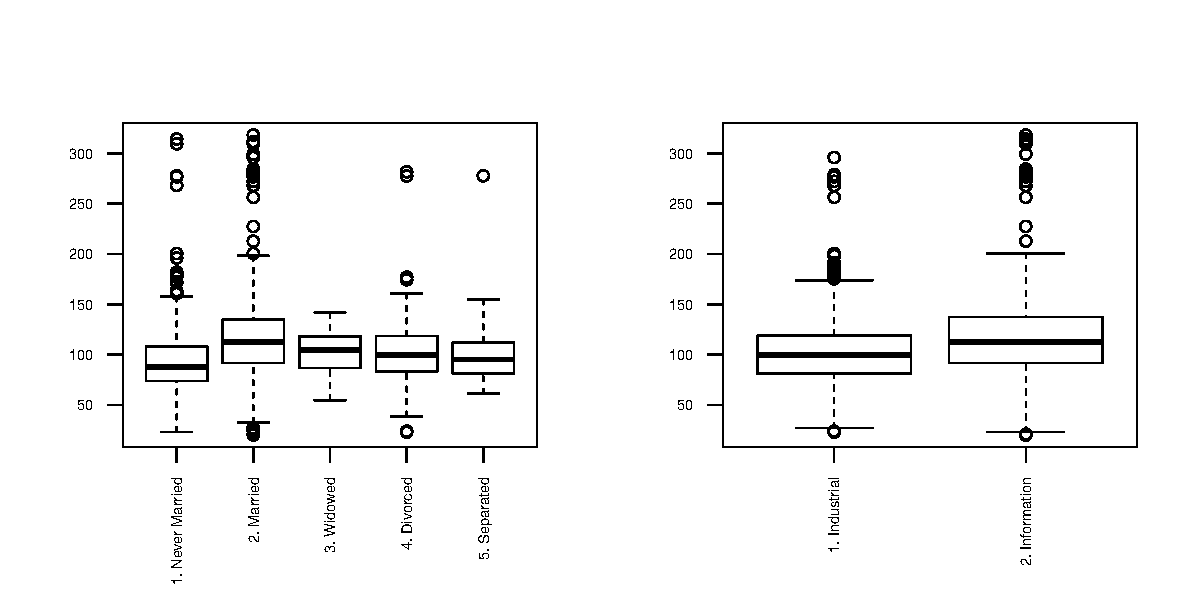
\includegraphics[width=0.8\textwidth]{MTH522_hw6_p2_1.pdf}
	\end{center}
	\caption{.}
	\label{fig:MTH522_hw6_p2_1}
\end{figure}

Conclusion: Plot 1, A married group earns more money on average. Plot 2, Informational jobs group earns more on average.




\newpage

\begin{program}
	\begin{verbatim}
	> fit1 <- gam(wage ~ maritl, data = Wage)
	> fit2 <- gam(wage ~ jobclass, data = Wage)
	> fit3 <- gam(wage ~ maritl + jobclass, data = Wage)
	> fit4 <- gam(wage ~ maritl + jobclass + s(age, 5) , data = Wage)
	> fit5 <- gam(wage ~ maritl + jobclass + s(age, 5) + education , data = Wage)
	> anova(fit1, fit2, fit3, fit4, fit5)
	Analysis of Deviance Table
	
	Model 1: wage ~ maritl
	Model 2: wage ~ jobclass
	Model 3: wage ~ maritl + jobclass
	Model 4: wage ~ maritl + jobclass + s(age, 5)
	Model 5: wage ~ maritl + jobclass + s(age, 5) + education
	Resid. Df Resid. Dev      Df Deviance  Pr(>Chi)    
	1      2995    4858941                               
	2      2998    4998547 -3.0000  -139606 < 2.2e-16 ***
	3      2994    4654752  4.0000   343795 < 2.2e-16 ***
	4      2989    4472687  4.9997   182065 < 2.2e-16 ***
	5      2985    3604891  4.0000   867796 < 2.2e-16 ***
	---
	Signif. codes:  0 ‘***’ 0.001 ‘**’ 0.01 ‘*’ 0.05 ‘.’ 0.1 ‘ ’ 1	
	\end{verbatim}
\end{program}

As we can see "fit5 : maritl + jobclass + s(age, 5) + education" add statistically significant improvements to the model and significantly better.





\begin{program}
	\begin{verbatim}
	> fit1 <- gam(wage ~ maritl, data = Wage)
	> fit2 <- gam(wage ~ jobclass, data = Wage)
	> fit3 <- gam(wage ~ maritl + jobclass, data = Wage)
	> fit4 <- gam(wage ~ maritl + jobclass + s(age, 5) , data = Wage)
	> fit5 <- gam(wage ~ maritl + jobclass + s(age, 5) + education , data = Wage)
	> anova(fit1, fit2, fit3, fit4, fit5)
	Analysis of Deviance Table
	
	Model 1: wage ~ maritl
	Model 2: wage ~ jobclass
	Model 3: wage ~ maritl + jobclass
	Model 4: wage ~ maritl + jobclass + s(age, 5)
	Model 5: wage ~ maritl + jobclass + s(age, 5) + education
	Resid. Df Resid. Dev      Df Deviance  Pr(>Chi)    
	1      2995    4858941                               
	2      2998    4998547 -3.0000  -139606 < 2.2e-16 ***
	3      2994    4654752  4.0000   343795 < 2.2e-16 ***
	4      2989    4472687  4.9997   182065 < 2.2e-16 ***
	5      2985    3604891  4.0000   867796 < 2.2e-16 ***
	---
	Signif. codes:  0 ‘***’ 0.001 ‘**’ 0.01 ‘*’ 0.05 ‘.’ 0.1 ‘ ’ 1
	\end{verbatim}
\end{program}

\newpage


\begin{program}
	\begin{verbatim}
	> par(mfrow = c(2, 2), las=2,cex.axis = 0.6)
	> plot(fit5, se = T, col = "blue")
	> dev.copy2pdf(file = "MTH522_hw6_p2_2.pdf", width = 8, height = 6, out.type = "pdf")
	> dev.off()
	\end{verbatim}
\end{program}

\begin{figure}[htb]
	\begin{center}
		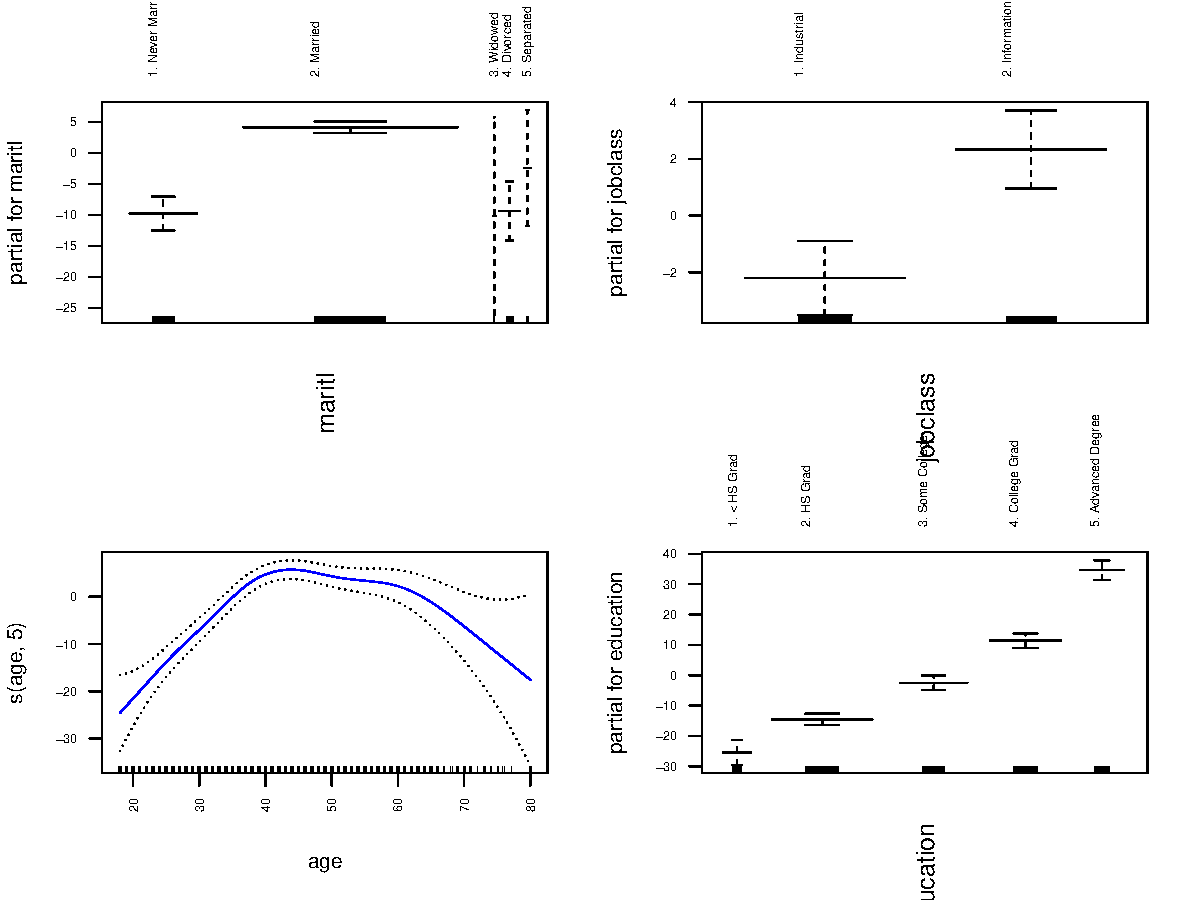
\includegraphics[width=0.8\textwidth]{MTH522_hw6_p2_2.pdf}
	\end{center}
	\caption{.}
	\label{fig:MTH522_hw6_p2_2}
\end{figure}

\newpage

{\bf Problem 3} (Chapter 7 Exercises 9):\\
This question uses the variables dis (the weighted mean of distances to five Boston employment centers) and nox (nitrogen oxides concen- tration in parts per 10 million) from the Boston data. We will treat dis as the predictor and nox as the response.\\
\\
(a) Use the poly() function to fit a cubic polynomial regression to predict nox using dis. Report the regression output, and plot the resulting data and polynomial fits.\\

\begin{program}
	\begin{verbatim}
	> set.seed(1)
	> library(MASS)
	> attach(Boston)
	> fit = lm(nox ~ poly(dis, 3), data = Boston)
	> summary(fit)
	
	Call:
	lm(formula = nox ~ poly(dis, 3), data = Boston)
	
	Residuals:
	Min        1Q    Median        3Q       Max 
	-0.121130 -0.040619 -0.009738  0.023385  0.194904 
	
	Coefficients:
	Estimate Std. Error t value Pr(>|t|)    
	(Intercept)    0.554695   0.002759 201.021  < 2e-16 ***
	poly(dis, 3)1 -2.003096   0.062071 -32.271  < 2e-16 ***
	poly(dis, 3)2  0.856330   0.062071  13.796  < 2e-16 ***
	poly(dis, 3)3 -0.318049   0.062071  -5.124 4.27e-07 ***
	---
	Signif. codes:  0 ‘***’ 0.001 ‘**’ 0.01 ‘*’ 0.05 ‘.’ 0.1 ‘ ’ 1
	
	Residual standard error: 0.06207 on 502 degrees of freedom
	Multiple R-squared:  0.7148,	Adjusted R-squared:  0.7131 
	F-statistic: 419.3 on 3 and 502 DF,  p-value: < 2.2e-16
	
	\end{verbatim}
\end{program}


\begin{program}
	\begin{verbatim}
	> dislim = range(dis)
	> grid = seq(from = dislim[1], to = dislim[2], by = 0.1)
	> pred = predict(fit, list(dis = grid))
	> plot(nox ~ dis, data = Boston, col = "darkgrey")
	> lines(grid, pred, col = "red", lwd = 2)
	> dislim = range(dis)
	> grid = seq(from = dislim[1], to = dislim[2], by = 0.1)
	> pred = predict(fit, list(dis = grid))
	> plot(nox ~ dis, data = Boston, col = "darkgrey")
	> lines(grid, pred, col = "red", lwd = 2)
	> dev.copy2pdf(file = "MTH522_hw6_p3a_1.pdf", width = 8, height = 6, out.type = "pdf")
	> dev.off()
	\end{verbatim}
\end{program}

\newpage


\begin{figure}[htb]
	\begin{center}
		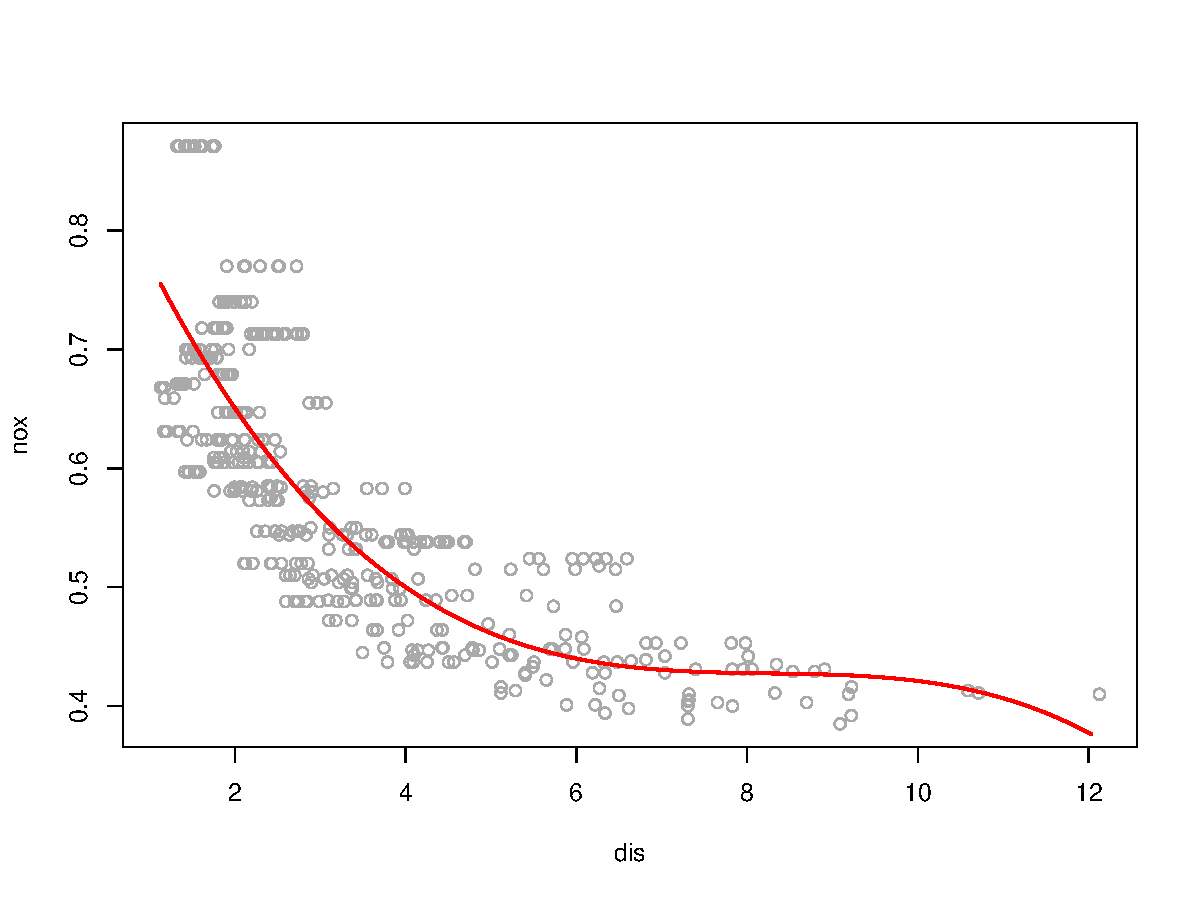
\includegraphics[width=0.8\textwidth]{MTH522_hw6_p3a_1.pdf}
	\end{center}
	\caption{.}
	\label{fig:MTH522_hw6_p3a_1}
\end{figure}

I used the poly() function "nox ~ poly(dis, 3)"  to fit a cubic polynomial regression to predict nox using dis and find out that all polynomial terms are significant while predicting nox using dis. As you can see, above  figure shows that a smooth curve fitting the data well.\\


\newpage 

(b) Plot the polynomial fits for a range of different polynomial degrees (say, from 1 to 10), and report the associated residual sum of squares.\\
\\
Let's plot  polynomial degrees from 1 to 10 and report the associated residual sum of squares (RSS).


\begin{program}
	\begin{verbatim}
	> all.rss = rep(NA, 10)
	> for (i in 1:10) {
	+     fit = lm(nox ~ poly(dis, i), data = Boston)
	+     all.rss[i] = sum(fit$residuals^2)
	+ }
	> all.rss
	[1] 2.768563 2.035262 1.934107 1.932981 1.915290 1.878257 1.849484 1.835630 1.833331 1.832171
	
	> plot(1:10, all.rss, xlab = "Degree", ylab = "RSS", type = "l")
	> dev.copy2pdf(file = "MTH522_hw6_p3b.pdf", width = 8, height = 6, out.type = "pdf")
	> dev.off()
	\end{verbatim}
\end{program}


\begin{figure}[htb]
	\begin{center}
		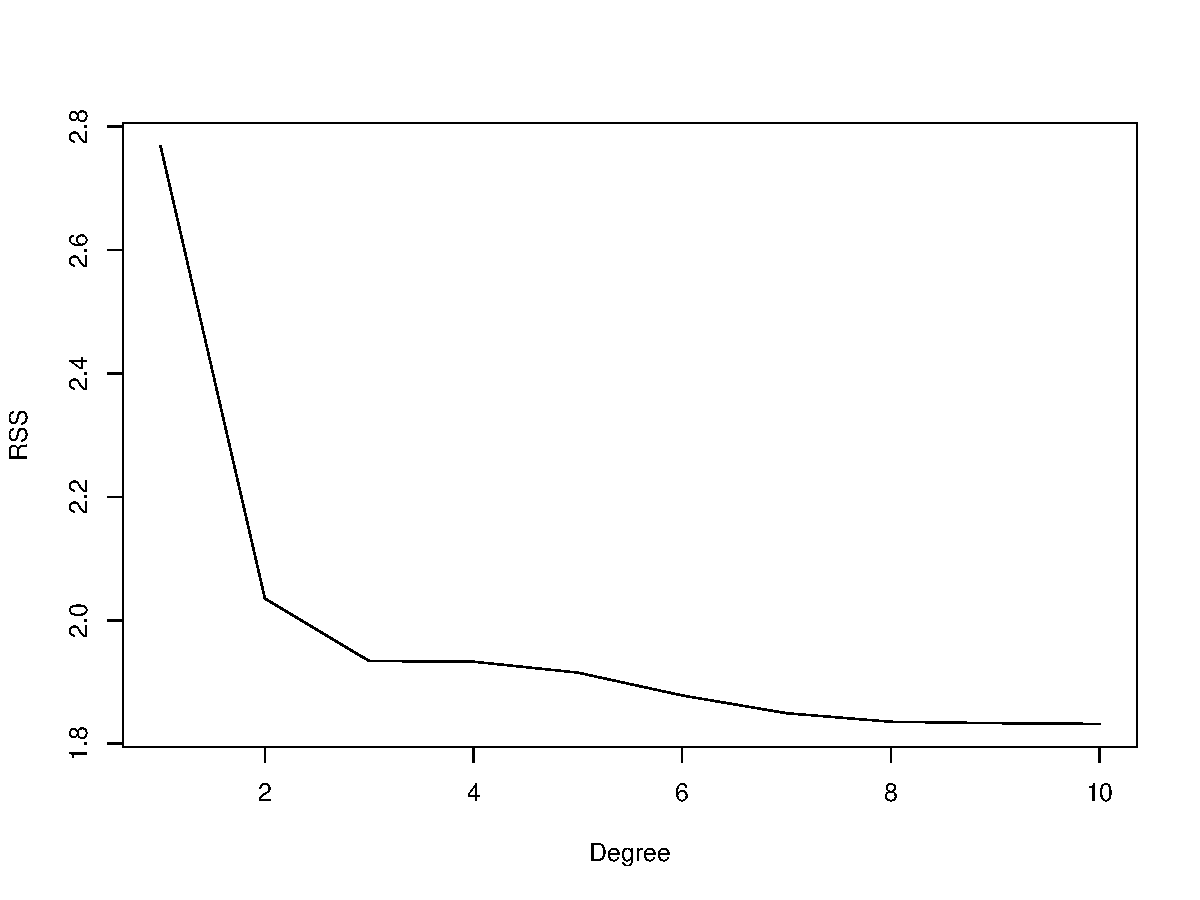
\includegraphics[width=0.8\textwidth]{MTH522_hw6_p3b.pdf}
	\end{center}
	\caption{.}
	\label{fig:MTH522_hw6_p3b}
\end{figure}

From plot, minimum for a polynomial of degree 10. RSS decreases with the degree of polinomial.

\newpage

(c) Perform cross-validation or another approach to select the optimal degree for the polynomial, and explain your results.\\

\begin{program}
	\begin{verbatim}
	> library(boot)
	> all.deltas = rep(NA, 10)
	> for (i in 1:10) {
	+     fit = glm(nox ~ poly(dis, i), data = Boston)
	+     all.deltas[i] = cv.glm(Boston, fit, K = 10)$delta[1]
	+ }
	> plot(1:10, all.deltas, xlab = "Degree", ylab = "CV Test error", type = "l")
	> 	dev.copy2pdf(file = "MTH522_hw6_p3c.pdf", width = 8, height = 6, out.type = "pdf")
	> 	dev.off()


	> which.min(all.deltas)
	[1] 4
	\end{verbatim}
\end{program}


\begin{figure}[htb]
	\begin{center}
		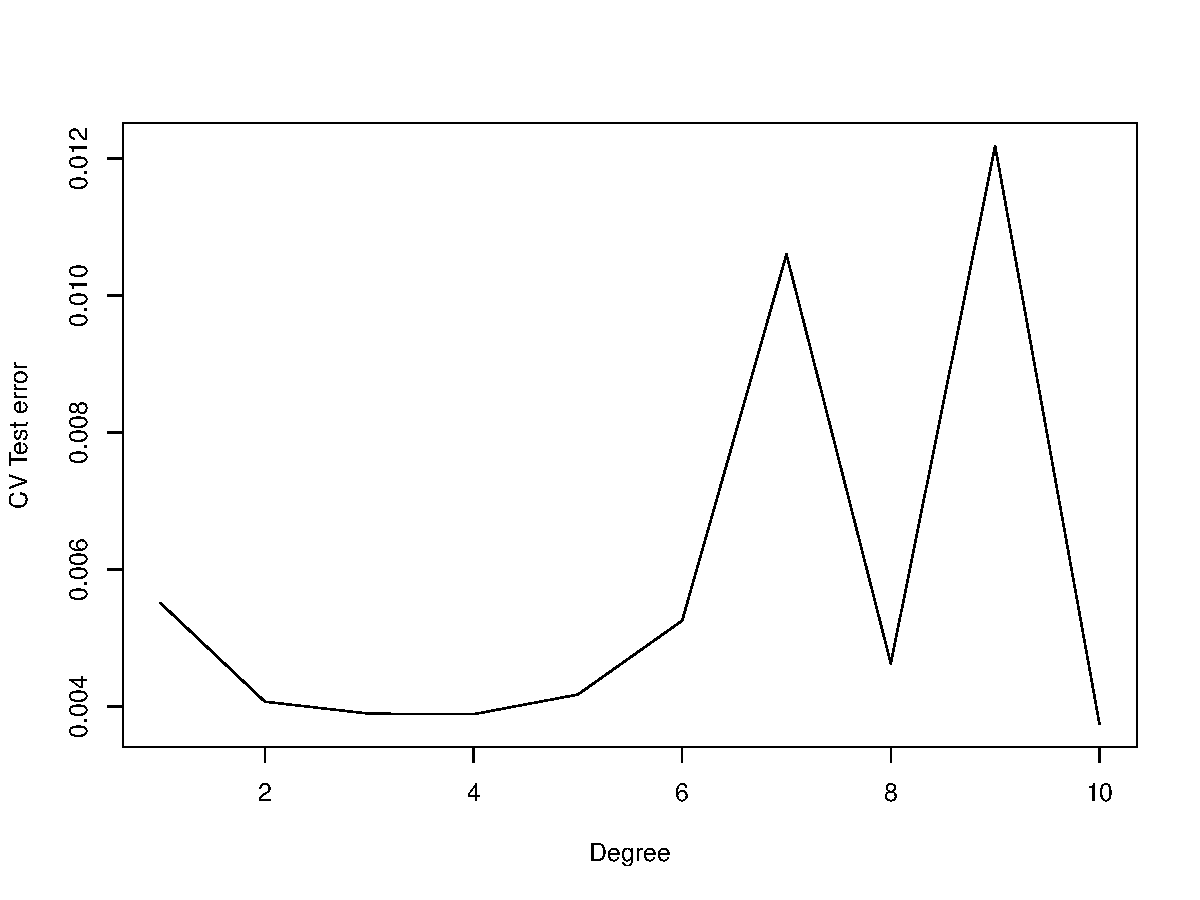
\includegraphics[width=0.8\textwidth]{MTH522_hw6_p3c.pdf}
	\end{center}
	\caption{.}
	\label{fig:MTH522_hw6_p3c}
\end{figure}

As we may see CV test error minimizes at the optimal degree for the polynomial 4. The error reduces between 1 to 3. From 3 to 4 reduces just little bit and after 4 start increasing for higher degrees.

\newpage


(d) Use the bs() function to fit a regression spline to predict nox using dis. Report the output for the fit using four degrees of freedom. How did you choose the knots? Plot the resulting fit.\\

\begin{program}
	\begin{verbatim}
	> library(splines)
	> fit = lm(nox ~ bs(dis, df = 4, knots = c(4, 7, 11)), data = Boston)
	> summary(fit)
	
	Call:
	lm(formula = nox ~ bs(dis, df = 4, knots = c(4, 7, 11)), data = Boston)
	
	Residuals:
	Min        1Q    Median        3Q       Max 
	-0.124567 -0.040355 -0.008702  0.024740  0.192920 
	
	Coefficients:
	Estimate Std. Error t value Pr(>|t|)    
	(Intercept)                            0.73926    0.01331  55.537  < 2e-16 ***
	bs(dis, df = 4, knots = c(4, 7, 11))1 -0.08861    0.02504  -3.539  0.00044 ***
	bs(dis, df = 4, knots = c(4, 7, 11))2 -0.31341    0.01680 -18.658  < 2e-16 ***
	bs(dis, df = 4, knots = c(4, 7, 11))3 -0.26618    0.03147  -8.459 3.00e-16 ***
	bs(dis, df = 4, knots = c(4, 7, 11))4 -0.39802    0.04647  -8.565  < 2e-16 ***
	bs(dis, df = 4, knots = c(4, 7, 11))5 -0.25681    0.09001  -2.853  0.00451 ** 
	bs(dis, df = 4, knots = c(4, 7, 11))6 -0.32926    0.06327  -5.204 2.85e-07 ***
	---
	Signif. codes:  0 ‘***’ 0.001 ‘**’ 0.01 ‘*’ 0.05 ‘.’ 0.1 ‘ ’ 1
	
	Residual standard error: 0.06185 on 499 degrees of freedom
	Multiple R-squared:  0.7185,	Adjusted R-squared:  0.7151 
	F-statistic: 212.3 on 6 and 499 DF,  p-value: < 2.2e-16
	
	
	
	
	> pred = predict(fit, list(dis = grid))
	> plot(nox ~ dis, data = Boston, col = "darkgrey")
	> lines(grid, pred, col = "red", lwd = 2)
	> dev.copy2pdf(file = "MTH522_hw6_p3d.pdf", width = 8, height = 6, out.type = "pdf")
	> dev.off()
	\end{verbatim}
\end{program}

\newpage

\begin{figure}[htb]
	\begin{center}
		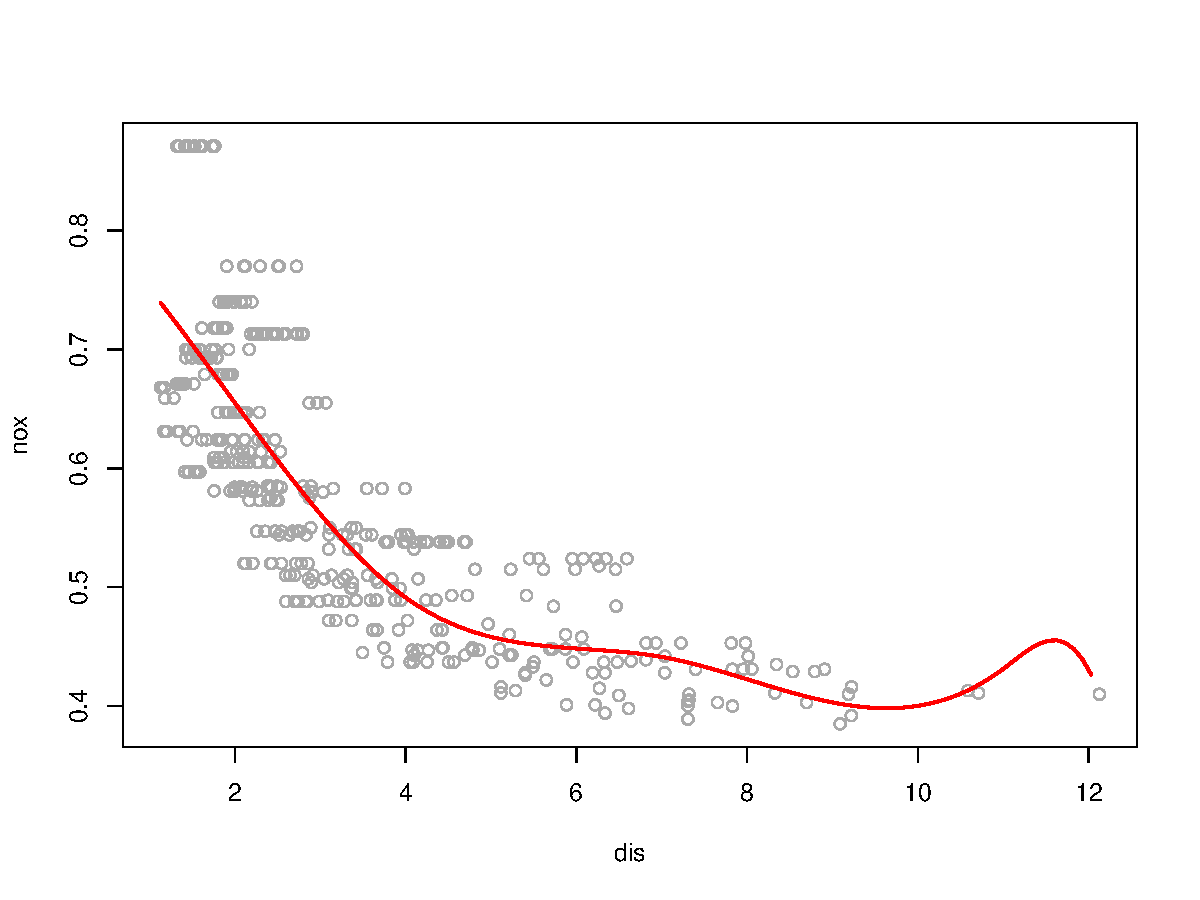
\includegraphics[width=0.8\textwidth]{MTH522_hw6_p3d.pdf}
	\end{center}
	\caption{.}
	\label{fig:MTH522_hw6_p3d}
\end{figure}

After using the bs() function to fit a regression splin and predict nox using dis, the plot shows that all terms in spline fit are significant except dis > 10 ecxtreme values.


\newpage


(e) Now fit a regression spline for a range of degrees of freedom, and plot the resulting fits and report the resulting RSS. Describe the results obtained.\\

\begin{program}
	\begin{verbatim}
	> rss = rep(NA, 16)
	> for (i in 3:16) {
	+     fit = lm(nox ~ bs(dis, df = i), data = Boston)
	+     rss[i] = sum(fit$residuals^2)   }
	> rss[-c(1, 2)]
	[1] 1.934107 1.922775 1.840173 1.833966 1.829884 1.816995 1.825653 1.792535 1.796992 1.788999
	[11] 1.782350 1.781838 1.782798 1.783546

	> which.min(rss)
	[1] 14
	> rss[which.min(rss)]
	[1] 1.781838

	> plot(3:16, rss[-c(1, 2)], xlab = "Degrees of freedom", ylab = "RSS", type = "l")
	> dev.copy2pdf(file = "MTH522_hw6_p3e.pdf", width = 8, height = 6, out.type = "pdf")
	> dev.off()
	\end{verbatim}
\end{program}


\begin{figure}[htb]
	\begin{center}
		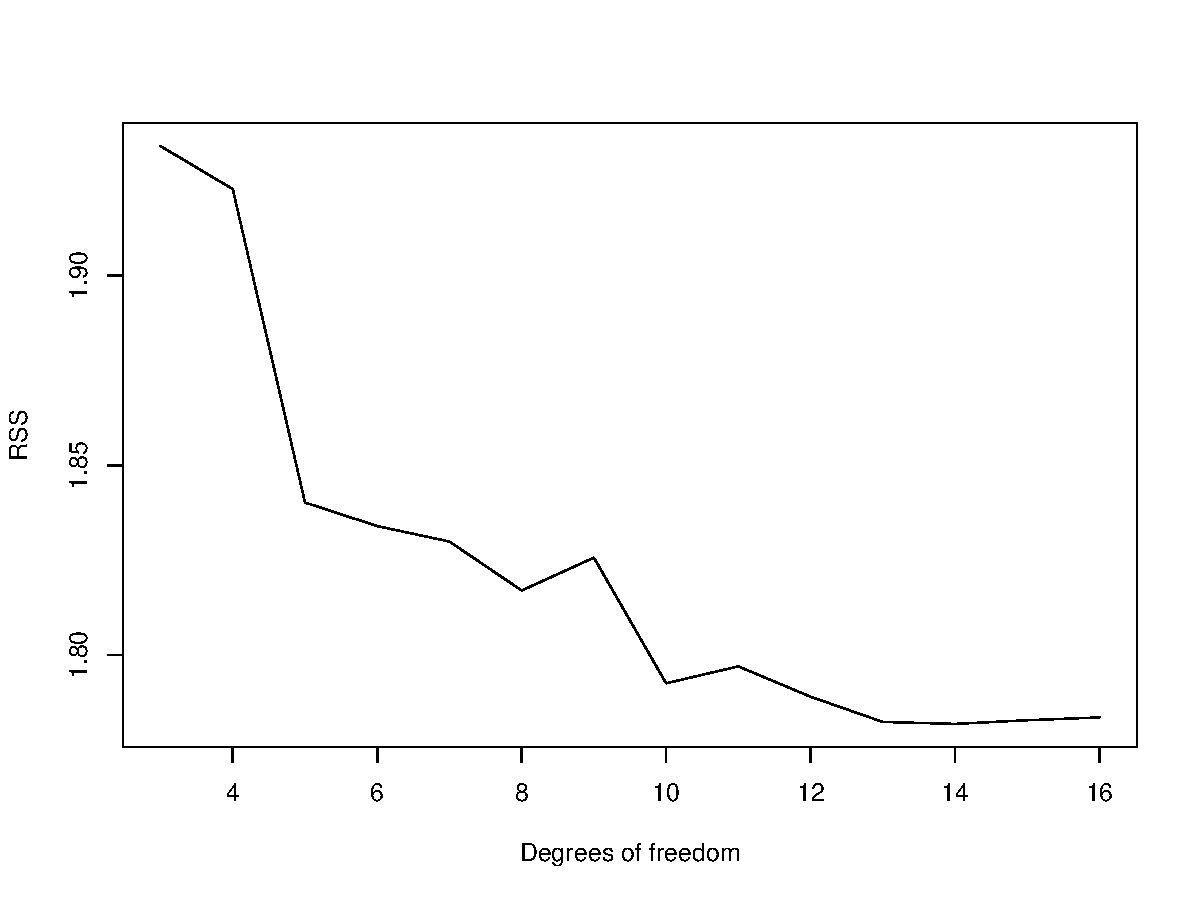
\includegraphics[width=0.8\textwidth]{MTH522_hw6_p3e.pdf}
	\end{center}
	\caption{.}
	\label{fig:MTH522_hw6_p3e}
\end{figure}


From plot, RSS decreases until 14 and then slightly increases after that.\\
\\
(f) Perform cross-validation or another approach in order to select the best degrees of freedom for a regression spline on this data. Describe your results.


\begin{program}
	\begin{verbatim}
	> cv = rep(NA, 16)
	> for (i in 3:16) {
	+     fit = glm(nox ~ bs(dis, df = i), data = Boston)
	+     cv[i] = cv.glm(Boston, fit, K = 10)$delta[2]
	+ }
	> cv[-c(1,2)]
	[1] 0.003853321 0.003883472 0.003730361 0.003704349 0.003687914 0.003695486 0.003750861
	[8] 0.003680307 0.003681417 0.003699190 0.003745600 0.003771265 0.003719676 0.003761896
	
	
	
	
	There were 50 warnings (use warnings() to see them)
	> warnings()
	Warning messages:
	1: In bs(dis, degree = 3L, knots = numeric(0), Boundary.knots = c(1.137,  ... :
	some 'x' values beyond boundary knots may cause ill-conditioned bases
	2: In bs(dis, degree = 3L, knots = numeric(0), Boundary.knots = c(1.137,  ... :
	some 'x' values beyond boundary knots may cause ill-conditioned bases
	3: In bs(dis, degree = 3L, knots = numeric(0), Boundary.knots = c(1.1296,  ... :
	some 'x' values beyond boundary knots may cause ill-conditioned bases
	4: In bs(dis, degree = 3L, knots = numeric(0), Boundary.knots = c(1.1296,  ... :
	some 'x' values beyond boundary knots may cause ill-conditioned bases
	5: In bs(dis, degree = 3L, knots = structure(3.2157, .Names = "50%"),  ... :
	some 'x' values beyond boundary knots may cause ill-conditioned bases
	6: In bs(dis, degree = 3L, knots = structure(3.2157, .Names = "50%"),  ... :
	some 'x' values beyond boundary knots may cause ill-conditioned bases
	7: In bs(dis, degree = 3L, knots = structure(3.1423, .Names = "50%"),  ... :
	some 'x' values beyond boundary knots may cause ill-conditioned bases
	8: In bs(dis, degree = 3L, knots = structure(3.1423, .Names = "50%"),  ... :
	some 'x' values beyond boundary knots may cause ill-conditioned bases
	9: In bs(dis, degree = 3L, knots = structure(c(2.35093333333333,  ... :
	some 'x' values beyond boundary knots may cause ill-conditioned bases
	10: In bs(dis, degree = 3L, knots = structure(c(2.35093333333333,  ... :
	some 'x' values beyond boundary knots may cause ill-conditioned bases
	11: In bs(dis, degree = 3L, knots = structure(c(2.4212, 4.36263333333333 ... :
	some 'x' values beyond boundary knots may cause ill-conditioned bases
	12: In bs(dis, degree = 3L, knots = structure(c(2.4212, 4.36263333333333 ... :
	some 'x' values beyond boundary knots may cause ill-conditioned bases
	13: In bs(dis, degree = 3L, knots = structure(c(2.1103, 3.2628,  ... :
	some 'x' values beyond boundary knots may cause ill-conditioned bases
	14: In bs(dis, degree = 3L, knots = structure(c(2.1103, 3.2628,  ... :
	some 'x' values beyond boundary knots may cause ill-conditioned bases
	15: In bs(dis, degree = 3L, knots = structure(c(2.08755, 3.2157,  ... :
	some 'x' values beyond boundary knots may cause ill-conditioned bases
	16: In bs(dis, degree = 3L, knots = structure(c(2.08755, 3.2157,  ... :
	some 'x' values beyond boundary knots may cause ill-conditioned bases
	17: In bs(dis, degree = 3L, knots = structure(c(1.9512, 2.59774,  ... :
	some 'x' values beyond boundary knots may cause ill-conditioned bases
	18: In bs(dis, degree = 3L, knots = structure(c(1.9512, 2.59774,  ... :
	some 'x' values beyond boundary knots may cause ill-conditioned bases
	19: In bs(dis, degree = 3L, knots = structure(c(1.94264, 2.7147,  ... :
	some 'x' values beyond boundary knots may cause ill-conditioned bases
	20: In bs(dis, degree = 3L, knots = structure(c(1.94264, 2.7147,  ... :
	some 'x' values beyond boundary knots may cause ill-conditioned bases
	21: In bs(dis, degree = 3L, knots = structure(c(1.85586666666667,  ... :
	some 'x' values beyond boundary knots may cause ill-conditioned bases
	22: In bs(dis, degree = 3L, knots = structure(c(1.85586666666667,  ... :
	some 'x' values beyond boundary knots may cause ill-conditioned bases
	23: In bs(dis, degree = 3L, knots = structure(c(1.86156666666667,  ... :
	some 'x' values beyond boundary knots may cause ill-conditioned bases
	24: In bs(dis, degree = 3L, knots = structure(c(1.86156666666667,  ... :
	some 'x' values beyond boundary knots may cause ill-conditioned bases
	25: In bs(dis, degree = 3L, knots = structure(c(1.75728571428571,  ... :
	some 'x' values beyond boundary knots may cause ill-conditioned bases
	26: In bs(dis, degree = 3L, knots = structure(c(1.75728571428571,  ... :
	some 'x' values beyond boundary knots may cause ill-conditioned bases
	27: In bs(dis, degree = 3L, knots = structure(c(1.794, 2.2222,  ... :
	some 'x' values beyond boundary knots may cause ill-conditioned bases
	28: In bs(dis, degree = 3L, knots = structure(c(1.794, 2.2222,  ... :
	some 'x' values beyond boundary knots may cause ill-conditioned bases
	29: In bs(dis, degree = 3L, knots = structure(c(1.7353625,  ... :
	some 'x' values beyond boundary knots may cause ill-conditioned bases
	30: In bs(dis, degree = 3L, knots = structure(c(1.7353625,  ... :
	some 'x' values beyond boundary knots may cause ill-conditioned bases
	31: In bs(dis, degree = 3L, knots = structure(c(1.734325,  ... :
	some 'x' values beyond boundary knots may cause ill-conditioned bases
	32: In bs(dis, degree = 3L, knots = structure(c(1.734325,  ... :
	some 'x' values beyond boundary knots may cause ill-conditioned bases
	33: In bs(dis, degree = 3L, knots = structure(c(1.66282222222222,  ... :
	some 'x' values beyond boundary knots may cause ill-conditioned bases
	34: In bs(dis, degree = 3L, knots = structure(c(1.66282222222222,  ... :
	some 'x' values beyond boundary knots may cause ill-conditioned bases
	35: In bs(dis, degree = 3L, knots = structure(c(1.65344444444444,  ... :
	some 'x' values beyond boundary knots may cause ill-conditioned bases
	36: In bs(dis, degree = 3L, knots = structure(c(1.65344444444444,  ... :
	some 'x' values beyond boundary knots may cause ill-conditioned bases
	37: In bs(dis, degree = 3L, knots = structure(c(1.63564, 1.94984,  ... :
	some 'x' values beyond boundary knots may cause ill-conditioned bases
	38: In bs(dis, degree = 3L, knots = structure(c(1.63564, 1.94984,  ... :
	some 'x' values beyond boundary knots may cause ill-conditioned bases
	39: In bs(dis, degree = 3L, knots = structure(c(1.62728, 1.94264,  ... :
	some 'x' values beyond boundary knots may cause ill-conditioned bases
	40: In bs(dis, degree = 3L, knots = structure(c(1.62728, 1.94264,  ... :
	some 'x' values beyond boundary knots may cause ill-conditioned bases
	41: In bs(dis, degree = 3L, knots = structure(c(1.61592727272727,  ... :
	some 'x' values beyond boundary knots may cause ill-conditioned bases
	42: In bs(dis, degree = 3L, knots = structure(c(1.61592727272727,  ... :
	some 'x' values beyond boundary knots may cause ill-conditioned bases
	43: In bs(dis, degree = 3L, knots = structure(c(1.63492727272727,  ... :
	some 'x' values beyond boundary knots may cause ill-conditioned bases
	44: In bs(dis, degree = 3L, knots = structure(c(1.63492727272727,  ... :
	some 'x' values beyond boundary knots may cause ill-conditioned bases
	45: In bs(dis, degree = 3L, knots = structure(c(1.5874, 1.81873333333333,  ... :
	some 'x' values beyond boundary knots may cause ill-conditioned bases
	46: In bs(dis, degree = 3L, knots = structure(c(1.5874, 1.81873333333333,  ... :
	some 'x' values beyond boundary knots may cause ill-conditioned bases
	47: In bs(dis, degree = 3L, knots = structure(c(1.61175833333333,  ... :
	some 'x' values beyond boundary knots may cause ill-conditioned bases
	48: In bs(dis, degree = 3L, knots = structure(c(1.61175833333333,  ... :
	some 'x' values beyond boundary knots may cause ill-conditioned bases
	49: In bs(dis, degree = 3L, knots = structure(c(1.5888, 1.8125,  ... :
	some 'x' values beyond boundary knots may cause ill-conditioned bases
	50: In bs(dis, degree = 3L, knots = structure(c(1.5888, 1.8125,  ... :
	some 'x' values beyond boundary knots may cause ill-conditioned bases
	\end{verbatim}
\end{program}

\newpage


\begin{program}
	\begin{verbatim}
	> which.min(cv)
	[1] 10
	>  cv[which.min(cv)]
	[1] 0.003680307
	
	
	> plot(3:16, cv[-c(1, 2)], xlab = "Degrees of freedom", ylab = "CV test error", type = "l")
	> dev.copy2pdf(file = "MTH522_hw6_p3f.pdf", width = 8, height = 6, out.type = "pdf")
	> dev.off()
	\end{verbatim}
\end{program}


\begin{figure}[htb]
	\begin{center}
		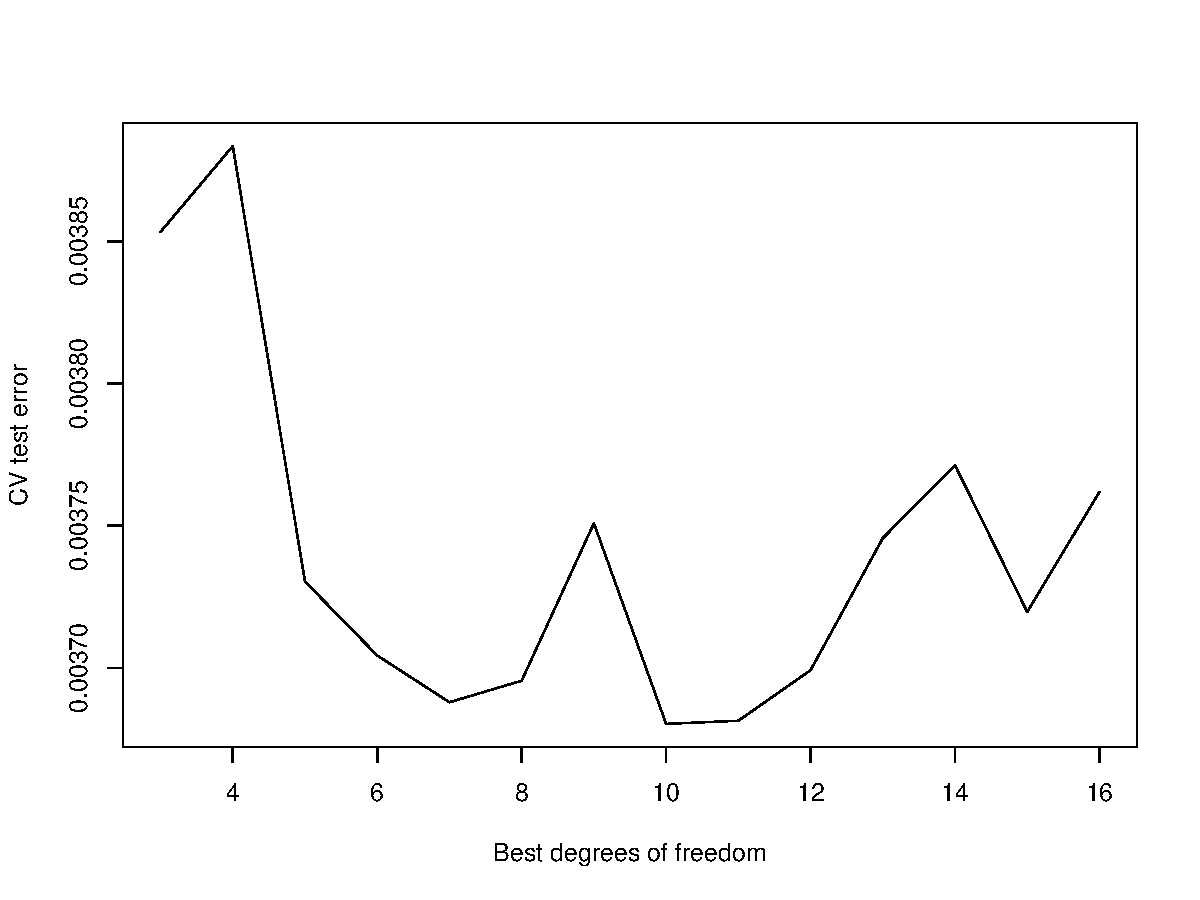
\includegraphics[width=0.8\textwidth]{MTH522_hw6_p3f.pdf}
	\end{center}
	\caption{.}
	\label{fig:MTH522_hw6_p3f}
\end{figure}

CV test error gets minimum af 10 the best degrees of freedom.

\newpage



{\bf Problem 4} (Chapter 7 Exercises 10):\\
This question relates to the College data set.\\

(a) Split the data into a training set and a test set. Using out-of-state tuition as the response and the other variables as the predictors, perform forward stepwise selection on the training set in order to identify a satisfactory model that uses just a subset of the predictors.\\

\begin{program}
	\begin{verbatim}
	> set.seed(1)
	>  library(ISLR)
	>  library(leaps)
	>  attach(College)
	> summary(College)
	Private        Apps           Accept          Enroll       Top10perc       Top25perc    
	No :212   Min.   :   81   Min.   :   72   Min.   :  35   Min.   : 1.00   Min.   :  9.0  
	Yes:565   1st Qu.:  776   1st Qu.:  604   1st Qu.: 242   1st Qu.:15.00   1st Qu.: 41.0  
	Median : 1558   Median : 1110   Median : 434   Median :23.00   Median : 54.0  
	Mean   : 3002   Mean   : 2019   Mean   : 780   Mean   :27.56   Mean   : 55.8  
	3rd Qu.: 3624   3rd Qu.: 2424   3rd Qu.: 902   3rd Qu.:35.00   3rd Qu.: 69.0  
	Max.   :48094   Max.   :26330   Max.   :6392   Max.   :96.00   Max.   :100.0  
	F.Undergrad     P.Undergrad         Outstate       Room.Board       Books       
	Min.   :  139   Min.   :    1.0   Min.   : 2340   Min.   :1780   Min.   :  96.0  
	1st Qu.:  992   1st Qu.:   95.0   1st Qu.: 7320   1st Qu.:3597   1st Qu.: 470.0  
	Median : 1707   Median :  353.0   Median : 9990   Median :4200   Median : 500.0  
	Mean   : 3700   Mean   :  855.3   Mean   :10441   Mean   :4358   Mean   : 549.4  
	3rd Qu.: 4005   3rd Qu.:  967.0   3rd Qu.:12925   3rd Qu.:5050   3rd Qu.: 600.0  
	Max.   :31643   Max.   :21836.0   Max.   :21700   Max.   :8124   Max.   :2340.0  
	Personal         PhD            Terminal       S.F.Ratio      perc.alumni   
	Min.   : 250   Min.   :  8.00   Min.   : 24.0   Min.   : 2.50   Min.   : 0.00  
	1st Qu.: 850   1st Qu.: 62.00   1st Qu.: 71.0   1st Qu.:11.50   1st Qu.:13.00  
	Median :1200   Median : 75.00   Median : 82.0   Median :13.60   Median :21.00  
	Mean   :1341   Mean   : 72.66   Mean   : 79.7   Mean   :14.09   Mean   :22.74  
	3rd Qu.:1700   3rd Qu.: 85.00   3rd Qu.: 92.0   3rd Qu.:16.50   3rd Qu.:31.00  
	Max.   :6800   Max.   :103.00   Max.   :100.0   Max.   :39.80   Max.   :64.00  
	Expend        Grad.Rate     
	Min.   : 3186   Min.   : 10.00  
	1st Qu.: 6751   1st Qu.: 53.00  
	Median : 8377   Median : 65.00  
	Mean   : 9660   Mean   : 65.46  
	3rd Qu.:10830   3rd Qu.: 78.00  
	Max.   :56233   Max.   :118.00  
	\end{verbatim}
\end{program}


\newpage

\begin{program}
	\begin{verbatim}
	> train = sample(length(Outstate), length(Outstate)/2)
	> test = -train
	> College.train = College[train, ]
	> College.test = College[test, ]
	> fit = regsubsets(Outstate ~ ., data = College.train, nvmax = 17, method = "forward")
	> summary = summary(reg.fit)

	> par(mfrow = c(1, 3))
	> plot(summary$cp, xlab = "Number of Variables", ylab = "Cp", type = "l")
	> min.cp = min(summary$cp)
	> std.cp = sd(summary$cp)
	> abline(h = min.cp + 0.2 * std.cp, col = "red", lty = 2)
	> abline(h = min.cp - 0.2 * std.cp, col = "red", lty = 2)

	> plot(reg.summary$bic, xlab = "Number of Variables", ylab = "BIC", type = "l")
	> min.bic = min(summary$bic)
	> std.bic = sd(summary$bic)
	> abline(h = min.bic + 0.2 * std.bic, col = "red", lty = 2)
	> abline(h = min.bic - 0.2 * std.bic, col = "red", lty = 2)

	> plot(summary$adjr2, xlab = "Number of Variables", ylab = "Adjusted R2",
	+     type = "l", ylim = c(0.4, 0.84))
	> max.adjr2 = max(summary$adjr2)
	> std.adjr2 = sd(summary$adjr2)
	> abline(h = max.adjr2 + 0.2 * std.adjr2, col = "red", lty = 2)
	> abline(h = max.adjr2 - 0.2 * std.adjr2, col = "red", lty = 2)
	> dev.copy2pdf(file = "MTH522_hw6_p4a.pdf", width = 8, height = 6, out.type = "pdf")
	> dev.off()
	\end{verbatim}
\end{program}



\begin{figure}[htb]
	\begin{center}
		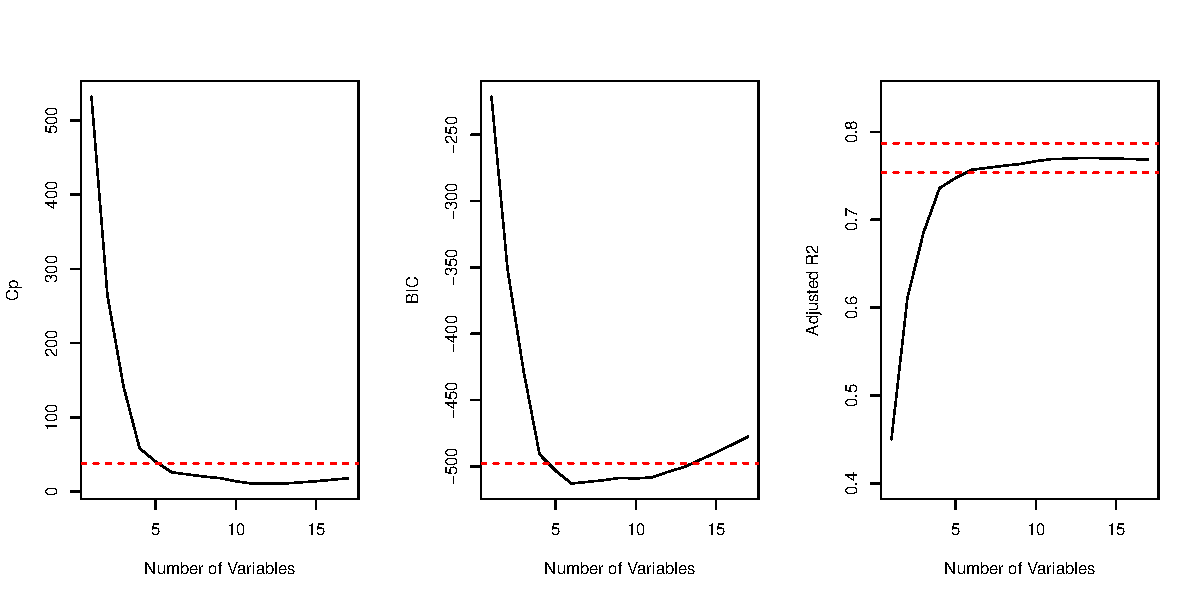
\includegraphics[width=0.8\textwidth]{MTH522_hw6_p4a.pdf}
	\end{center}
	\caption{.}
	\label{fig:MTH522_hw6_p4a}
\end{figure}


We are tryin to find the minimum size for the subset for which the scores are within 0.2 standard devitations of optimum.From the plot, Cp, BIC and adjr2 show that size should be bigger than 5,so we may see that number of veriables 6 is the minimum size. Let's see the best 6 veriables;


\begin{program}
	\begin{verbatim}
	> fit = regsubsets(Outstate ~ ., data = College, method = "forward")
	> coefi = coef(fit, id = 6)
	> names(coefi)
	[1] "(Intercept)" "PrivateYes"  "Room.Board"  "PhD"         "perc.alumni" "Expend"     
	[7] "Grad.Rate"  
	\end{verbatim}
\end{program}


\newpage


(b) Fit a GAM on the training data, using out-of-state tuition as the response and the features selected in the previous step as the predictors. Plot the results, and explain your findings.\\

\begin{program}
	\begin{verbatim}
	> fit = gam(Outstate ~ Private + s(Room.Board, df = 2) + s(PhD, df = 2) +
	+      s(perc.alumni, df = 2) + s(Expend, df = 5) + s(Grad.Rate, df = 2), data = College.train)
	>  par(mfrow = c(2, 3))
	>  plot(fit, se = T, col = "blue")
	> dev.copy2pdf(file = "MTH522_hw6_p4b.pdf", width = 8, height = 6, out.type = "pdf")
	> dev.off()
	\end{verbatim}
\end{program}


\begin{figure}[htb]
	\begin{center}
		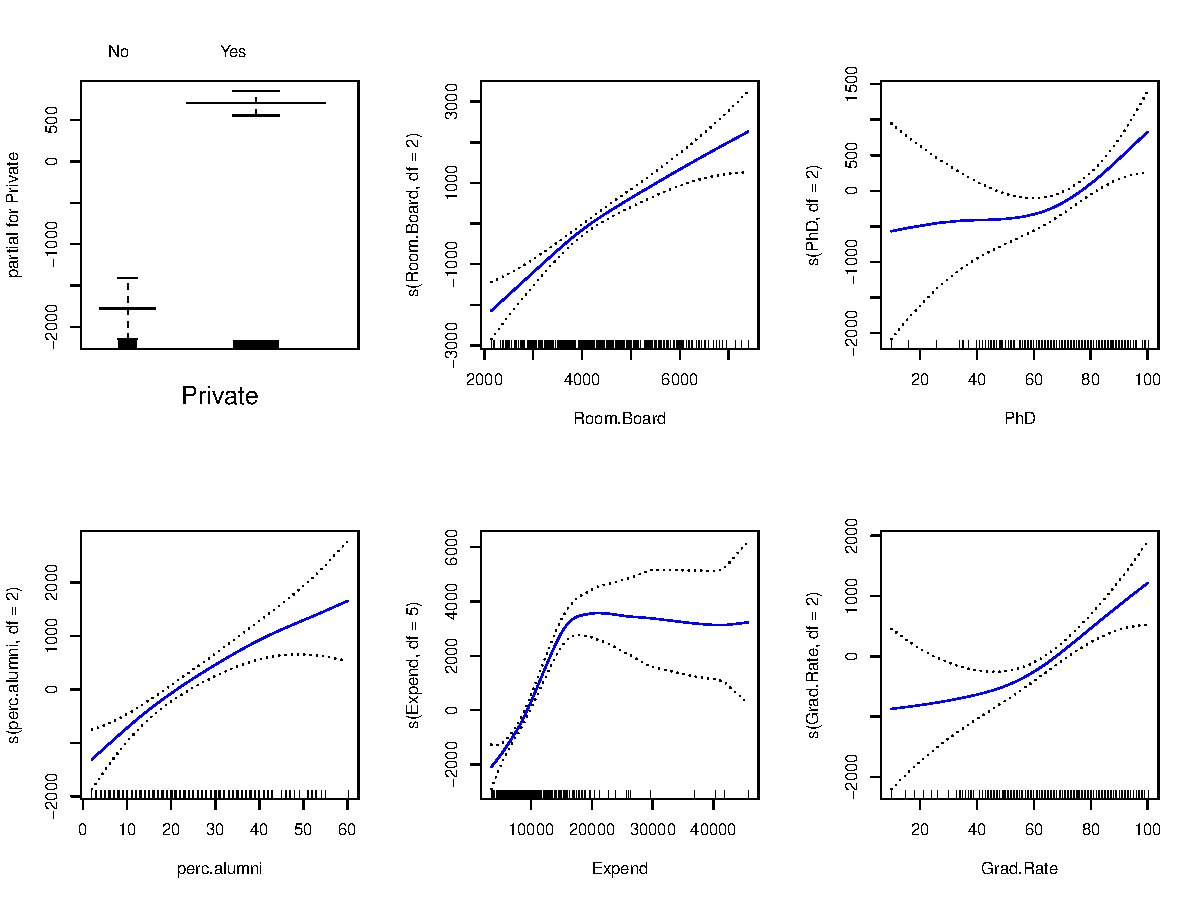
\includegraphics[width=0.8\textwidth]{MTH522_hw6_p4b.pdf}
	\end{center}
	\caption{.}
	\label{fig:MTH522_hw6_p4b}
\end{figure}

\newpage


(c) Evaluate the model obtained on the test set, and explain the results obtained.\\

\begin{program}
	\begin{verbatim}
	> pred = predict(fit, College.test)
	> err = mean((College.test$Outstate - pred)^2)
	> err
	[1] 3745460




	> tss = mean((College.test$Outstate - mean(College.test$Outstate))^2)
	> rss = 1 - err/tss
	> rss
	[1] 0.7696916
	\end{verbatim}
\end{program}

After evaluation the model obtained on the test set, we optain $R^2$ of 0.7696916 using GAM with 6 predictors.


\newpage

(d) For which variables, if any, is there evidence of a non-linear relationship with the response?


\begin{program}
	\begin{verbatim}
	> summary(fit)
	
	Call: gam(formula = Outstate ~ Private + s(Room.Board, df = 2) + s(PhD, 
	df = 2) + s(perc.alumni, df = 2) + s(Expend, df = 5) + s(Grad.Rate, 
	df = 2), data = College.train)
	Deviance Residuals:
	Min       1Q   Median       3Q      Max 
	-4977.74 -1184.52    58.33  1220.04  7688.30 
	
	(Dispersion Parameter for gaussian family taken to be 3300711)
	
	Null Deviance: 6221998532 on 387 degrees of freedom
	Residual Deviance: 1231165118 on 373 degrees of freedom
	AIC: 6941.542 
	
	Number of Local Scoring Iterations: 2 
	
	Anova for Parametric Effects
	Df     Sum Sq    Mean Sq F value    Pr(>F)    
	Private                  1 1779433688 1779433688 539.106 < 2.2e-16 ***
	s(Room.Board, df = 2)    1 1221825562 1221825562 370.171 < 2.2e-16 ***
	s(PhD, df = 2)           1  382472137  382472137 115.876 < 2.2e-16 ***
	s(perc.alumni, df = 2)   1  328493313  328493313  99.522 < 2.2e-16 ***
	s(Expend, df = 5)        1  416585875  416585875 126.211 < 2.2e-16 ***
	s(Grad.Rate, df = 2)     1   55284580   55284580  16.749 5.232e-05 ***
	Residuals              373 1231165118    3300711                      
	---
	Signif. codes:  0 ‘***’ 0.001 ‘**’ 0.01 ‘*’ 0.05 ‘.’ 0.1 ‘ ’ 1
	
	Anova for Nonparametric Effects
	Npar Df  Npar F     Pr(F)    
	(Intercept)                                         
	Private                                             
	s(Room.Board, df = 2)        1  3.5562   0.06010 .  
	s(PhD, df = 2)               1  4.3421   0.03786 *  
	s(perc.alumni, df = 2)       1  1.9158   0.16715    
	s(Expend, df = 5)            4 16.8636 1.016e-12 ***
	s(Grad.Rate, df = 2)         1  3.7208   0.05450 .  
	---
	Signif. codes:  0 ‘***’ 0.001 ‘**’ 0.01 ‘*’ 0.05 ‘.’ 0.1 ‘ ’ 1
	\end{verbatim}
\end{program}

Anova for Nonparametric shows that there is a strong evidence of non-linear relationship between "Outstate" and "Expend".
Using p value of 0.05, there is a moderatly strong non-linear relationship between "Outstate" and "PhD" or "Grad.Rate".


\end{document}





